\documentclass[conference]{IEEEtran}
\IEEEoverridecommandlockouts
% The preceding line is only needed to identify funding in the first footnote. If that is unneeded, please comment it out.
\usepackage{amsmath,amssymb,amsfonts}
\usepackage{algorithmic}
\usepackage{graphicx}
\usepackage{textcomp}
\usepackage{xcolor}
\usepackage{comment}
%%%%%%%%%%%%%%%%%%%%%%%%%%%%%%%%%%%%%%%%%%%%%%%%%%%%%%%%%
%%%%%%%%%%%%%%%%%%%%%%%%%%%%%%%%%%%%%%%%%%%%%%%%%%%%%%%%%
%%%%%%%%%%%%%%%%%%%%%%%%%%%%%%%%%%%%%%%%%%%%%%%%%%%%%%%%%
%%%%%%% REMOVE FOLLOWING LINE BEFORE SUBMITTING %%%%%%%%%
\setlength {\marginparwidth }{2cm}
%%%%%%%%%%%%%%%%%%%%%%%%%%%%%%%%%%%%%%%%%%%%%%%%%%%%%%%%%
%%%%%%%%%%%%%%%%%%%%%%%%%%%%%%%%%%%%%%%%%%%%%%%%%%%%%%%%%
%%%%%%%%%%%%%%%%%%%%%%%%%%%%%%%%%%%%%%%%%%%%%%%%%%%%%%%%%
%%%%%%%%%%%%%%%%%%%%%%%%%%%%%%%%%%%%%%%%%%%%%%%%%%%%%%%%%
\usepackage{todonotes}
\usepackage{wrapfig}
\usepackage{hyperref}
\usepackage{xurl}
\usepackage{booktabs}
\usepackage{float}
\usepackage[noadjust]{cite}

\def\BibTeX{{\rm B\kern-.05em{\sc i\kern-.025em b}\kern-.08em
    T\kern-.1667em\lower.7ex\hbox{E}\kern-.125emX}}
\begin{document}

\title{Automated Metadata Generation for Fish Specimen Image Collections%*\\
    {\footnotesize \thanks{NSF Grant ???} }}

\author{
\IEEEauthorblockN{Joel Pepper}
\IEEEauthorblockA{\textit{Department of Computer Science} \\
\textit{Drexel University}\\
Philadelphia, USA\\
0000-0002-1601-8729}
\and
\IEEEauthorblockN{Jane Greenberg}
\IEEEauthorblockA{\textit{Department of Information Science} \\
\textit{Drexel University}\\
Philadelphia, USA\\
0000-0001-7819-5360}
\and
\IEEEauthorblockN{Yasin Baki\c{s}}
\IEEEauthorblockA{\textit{Biodiversity Research Institute} \\
\textit{Tulane University}\\
New Orleans, USA\\
0000-0001-6144-9440}
\and
\IEEEauthorblockN{Xiaojun Wang}
\IEEEauthorblockA{\textit{Biodiversity Research Institute} \\
\textit{Tulane University}\\
New Orleans, USA\\
0000-0001-8639-6795}
\and
\IEEEauthorblockN{Henry Bart Jr.}
\IEEEauthorblockA{\textit{Biodiversity Research Institute} \\
\textit{Tulane University}\\
New Orleans, USA\\
0000-0002-5662-9444}
\and
\IEEEauthorblockN{David Breen}
\IEEEauthorblockA{\textit{Department of Computer Science} \\
\textit{Drexel University}\\
Philadelphia, USA\\
0000-0002-1376-5008}
}

\maketitle

\begin{abstract}
     Over the last several decades advances in computing, imaging, and cyberinfrastructure have had a major impact on scientific research and discovery. One area of considerable activity is the digitization of the biological specimens that have been acquired worldwide by museums and other research institutions, undertakings that have produced large image collections.
The metadata that is vital for subsequent machine learning, analysis and
scientific discovery based on these specimen image repositories
is often unavailable, sparse or incorrect.
As a step towards improving metadata in specimen research image collections, our team is developing methods for automatically analyzing fish images to extract a variety of important features. These fish specimens are being studied for a larger project entitled Biology Guided Neural Networks (BGNN), which is developing a novel class of artificial neural networks that can exploit the machine readable and predictive knowledge about biology that is available in specimen images, phylogenies and anatomy ontologies. Using a combination of machine learning and image informatics tools and techniques, we can accurately determine metadata such as fish quantity and location within images, fish orientation and other quantitative fish features, image scaling based on ruler identification and measurement, and general image quality metrics for a substantial number of the images being used in the BGNN project.
Our goal is to develop image metadata generation methods that both support
the research underway within the BGNN project, and provide a framework for future technology developments that can be deployed by repository curators to improve and bolster the metadata they provide with their specimen images. A longer term goal is to extend the image analysis methods for computing quantitative features in support of specific biological investigations.
\end{abstract}

\begin{IEEEkeywords}
bioinformatics, metadata, image analysis, applied machine learning
\end{IEEEkeywords}

\section{Introduction}
% Moving teaser since this template doesn't actually ask for one
Over the last several decades advances in computing, imaging, and cyberinfrastructure have supported the growth of digital natural history collections, many of which have specimen images.~\cite{beaman2012mass} Additionally, initiatives, such as National Science Foundation’s Advancing Digitization of Biodiversity Collections (ADBC) program, which ran for nearly a decade, have supported the digitization and curation of tens of thousands of biological specimens.~\cite{page2015digitization} These digital specimen accessible through global, open access repositories; they enable researchers, educators, students, and the general public to examine and compare in ways previously unimaginable. Significant challenges surface, however, when researchers seek to apply computational methods to these data items, due to both image quality and metadata issues.
%{jane}should we try to insert machine learning here, last sentence, or computation methods ok?

Unfortunately, potential scientific advances are hindered by image quality
problems and the lack of accurate and pertinent metadata
associated with the image collections.
Poor quality images, e.g. with low contrast, inadequate lighting,
out-of-focus or cluttered visual arrangements, provide inadequate input
for automated
image analysis and machine learning algorithms and lead to inferior
computational results.
In order to perform quantitative morphometric analysis of the specimens,
the physical scale of the images (pixels/inch) is needed; thus
requiring the ability to identify and measure rulers in the images.
Many specimen collections do include Darwin Core metadata,~\cite{biodiv_info_standards} detailing
specimen taxon, geographic location, and several other descriptive aspects.
Additionally, some digitization efforts record technical metadata, detailing imaging specifications. While these types of metadata are helpful for a
human examining several images at a time, they are insufficient for researchers seeking to apply computational methods to examine thousands of images
to determine if, for instance, a specific fish grows to different lengths
in different habitats.

Since the digital collections may each contain tens of thousands of images, producing metadata for each image via a manual process is prohibitively labor-intensive and infeasible. Methods for automatically computing metadata from images are therefore needed to fully exploit biological image repositories for scientific discovery.
As a step towards improving metadata in specimen research image collections, members of Drexel University's Metadata Research Center are developing methods to automatically analyze fish images and
extract a set of data features that provide important metadata about the
digitized specimen.
The research is being conducted as part of the Biology Guided Neural Networks (BGNN) project, which aims to develop a novel class of artificial neural networks that exploit machine readable and predictive knowledge associated with specimen images, phylogenies and anatomy ontologies.
Using a combination of machine learning and image informatics tools and techniques, we can accurately determine general image quality and metadata, such as fish quantity and location within images, fish orientation, and
image scaling based on ruler identification and measurement. Image scaling
allows us to compute quantitative features about the fish specimens, such
as their length and area.  In order to test and validate our methods, they
were  applied to a set of 7,247
images drawn from the Illinois Natural History Survey (INHS) Collection.
The following section of the paper provides contextual background for this work, followed by the research goals and objectives, and a review of our research methods. Next, the results are presented, followed by a discussion. The conclusion highlights key findings and identifies next steps.

\section{Related Work}
\textbf{Todo}
\subsection{Metadata for Natural History Image Collection}
%question/comment - we need to keep in mind we are deal with digitized specimens, not simply digital, in other words, the artifacts themselves are digital version of physical, not like an x-ray, where the image is digital from the start.  
A number of different metadata standards have been applied to support the description and access of digitized scientific images. Darwin Core developed specifically for digital museum projects is one of the most frequently used standards. Other popular standards include the Dublin Core, particularly application profiles, drawing from other namespaces such as the Ecological Metadata Language (EML) and ISO-geo [jane add]; and there is also the recent Audubon Core, designed to support the discoverability, dissemination, and use of data relating to biological organisms, including digitized specimens. These descriptive standards include metadata properties for taxon, geographic location, and other important specimen content, and have been developed primarily from the eye of a human curator. In other words, their application anticipates that a curator or data entry staff person will manually enter data from the original acquisition logs, or historical labels. As a result, the metadata associated with each digital rendering seems somewhat limited, particularly to researchers seeking to apply machine learning, and leverage both the image and the metadata.
%will add cites above, depending on paper length.

%Fish species dataset in Pakistan Shah 2019 \cite{Shah2019FishPakFS},

\subsection{Automatic Metadata Generation}
Metadata researchers are aware of challenges posted by manual metadata generation, both in terms of time, 
%jane working here, i figured out how to scope this, I think! I need to get outside now, but back later.

\subsection{Fish Image Analysis}

Image analysis has been utilized to examine and process images of fish
for well over two decades \cite{Zion2000InvivoFS,Saberioon2017ApplicationOM}. It is an important
application of technology both for marine science, in the study of aquatic
species, habitats and ecosystems, and for the seafood industry, in the
development of automated fish sorting and grading systems, as well as
fisheries management. Many of these computational analyses focus on
the recognition and classification
of the fish present in an image.  The computational methods employed for
fish image analysis have followed the general trends in the AI field.
Hu et al.~\cite{HuJing2012Fscb} presented a method of classifying species
of fish based on color and texture features and a multi-class support
vector machine (MSVM) \cite{Vapnik1999AOS}.
Li and Hong \cite{Li2014IdentificationOF} computed eleven shape and color
features from fish images that were distilled down to four, using Principal
Component Analysis, and derived a linear model
that could discriminate between four different fishes.
%  Kinda unimpressive. Let's leave out.
% Saitoh \cite{Saitoh2015ImagebasedFR}
% utilized a Random Forest method \cite{Breiman2001RF} on manually-derived
% geometric, Bag of visual words (BoVW) and color features 
Rodrigues et al.~\cite{RodriguesMarcoT.A2015Ecda} explored several
combinations of features extraction, input classifiers and clustering
algorithms to produce a method that could distinguish between 10 different
types of fish with a 92\% accuracy.
%  Again, not too impressive. Let's leave out.
% Ogunlana 2015 \cite{Ogunlana2015FCU},
% In this paper, a Support Vector Machine (SVM)-based technique for the elimination of the limitations of some existing techniques and improved classification of fish species is proposed. The technique is based on the shape features of fish that was divided into two subsets with the first comprising 76 fish as training set while the second comprises of 74 fish as testing set. The body and the five fin lengths; namely anal, caudal, dorsal, pelvic and pectoral were extracted in centimeter (cm). Results based on the new technique show a classification accuracy of 78.59%, which is significantly higher than what obtained for ANN, KNN and K-mean clustering-based algorithms.
Salman et al.~\cite{Salman2016FishSC} employed a deep Convolution Neural
Networks (CNN) \cite{LeCun2004LMG} together with classification based on
K-Nearest Neighbor and Support Vector Machines trained on the features
extracted by the CNN. They achieved 90\%
accuracy when identifying 15 different fish in challenging underwater
digital images.
% Unimpressive. Do not include.
% Sung 2017 \cite{Sung2017VisionBR},
% Underwater vision has specific characteristics such as high attenuation of lights, severe noise and haze in the images. For real-time fish detection using underwater vision, this paper proposes convolutional neural network based techniques based on You Only Look Once algorithm. Actual fish video images were used to evaluate the reliability and accuracy of the proposed method. As a result, the network recorded 93% classification accuracy, 0.634 intersection over union between predicted bounding box and ground truth, and 16.7 frames per second of fish detection. It also outperforms another fish detector using sliding window algorithm and classifier trained with histogram of oriented gradient features and support vector machine.
% Not digging it.
% Hasija 2017 \cite{Hasija2017FishSC},
% This paper proposes a novel method based on an improved image-set matching approach, which makes use of Graph-Embedding Discriminant Analysis. In contrast to the state-of-the-art methods, which operate on single input images, our method makes, use of explicit image set matching which renders it robust computationally.
% Not this one either
% Sayed 2018 \cite{SayedGehadIsmail2018AAFS},
% This paper proposed an automated fish species identification system based on a modified crow search optimization algorithm. Median filtering is applied for image smoothing and removing noise through reducing the variation of intensities between the neighbors. Then, a k-mean clustering algorithm is used to segment the fish image into multiple segments. Shape-based and texture-based feature extraction process for classification is presented. A new modified binary version of crow search algorithm is proposed to reduce the data dimensionality of the extracted features. Finally, support vector machine and decision trees are implemented for classification and the fish species are classified based on either their class including Actinopterygii and Chondrichthyes or based on their order. Total of 270 images with different species, classes and orders are used for evaluation of the proposed system. The experimental results show that the proposed system achieves the highest classification accuracy compared to state-of-the-art algorithms. Also, the results show that the overall fish species identification system obtains on average of 10 folds, 96% classification accuracy for classification based on class and 74% for classification based on fish order.
Utilizing texture, anchor points, and statistical measurements,
Alsmadi et al.~\cite{Alsmadi2019RFE} implemented fish
classification through a meta-heuristic algorithm known as Memetic Algorithm (Genetic Algorithm with Simulated Annealing) with back-propagation algorithm (MA-B Classifier). They were able to classify 24 fish families with 90\%
accuracy.
% Nope
% Sharmin 2019 \cite{Sharmin2019MVB},
% the new generation people of Bangladesh lacks the knowledge of local freshwater fish. For this problem, a solution has been found with the collaboration of vision-based technology. As a solution, a machine-vision based local freshwater fish recognition system is presented that can be proceed with an image of fish captured with a mobile or handheld device and recognize the fish in order to introduce the fish. To demonstrate the utility of the proposed expert system, several experiments are performed. At first, a set of fourteen features, which consists of four types of features, are presented. Then the color image has been converted into gray-scale image and the gray-scale histogram is formed. Image segmentation takes place using histogram-based method and then the features are extracted. PCA is used for decreasing the feature numbers. Three classifiers are used for recognizing fish, where SVM gives the highest accuracy showing a value of 94.2%.
%  I want to see the paper before I cite it.
% Banan 2020 \cite{Banan2020DeepLA}
% Hence, in this study, a deep learning neural network as a smart, real-time and non-destructive method was developed and applied to automate the identification of four economically important carp species namely common carp (Cyprinus carpio), grass carp (Ctenopharingodon idella), bighead carp (Hypophtalmichthys nobilis) and silver carp (Hypophthalmichthys molitrix). The obtained results proved that our approach, evaluated through 5-fold cross-validation, achieved the highest possible accuracy of 100 %. The achieved high level of classification accuracy was due to the ability of the suggested deep model to build a hierarchy of self-learned features, which was in accordance with the hierarchy of these fish’s identification keys. In conclusion, the proposed convolutional neural network (CNN)-based method has a single and generic trained architecture with promising performance for fish species identification.
Iqbal et al.~\cite{Iqbal2021AutomaticFS} used a modified
AlexNet \cite{AlexNet2012} model to classify six different fish species
with 90\% accuracy.
% In this paper, we presented an automated system for identification and classification of fish species. It helps the marine biologists to have greater understanding of the fish species and their habitats. The proposed model is based on deep convolutional neural networks. It uses a reduced version of AlexNet model comprises of four convolutional layers and two fully connected layers. A comparison is presented against the other deep learning models such as AlexNet and VGGNet. The four parameters are considered that is number of convolu- tional layers and number of fully-connected layers, number of iterations to achieve 100% accuracy on training data, batch size and dropout layer. The results show that the proposed and modified AlexNet model with less number of layers has achieved the testing accuracy of 90.48% while the original AlexNet model achieved 86.65% over the untrained bench- mark fish dataset. The inclusion of dropout layer has enhanced the overall performance of our proposed model. It contain less training images, less memory and it is also less compu- tational complex.
%  No paper. No reference
% Xu 2021 \cite{Xu2021TransferLA},
% Scientific studies on species identification in fish have considerable significance in aquatic ecosystems and quality evaluation. The morphological differences between different fish species are obvious. Machine learning methods use artificial prior knowledge to extract fish features, which is time-consuming, laborious, and subjective. Recently, deep learning-based identification of fish species has been widely used. However, fish species identification still faces many challenges due to the small scale of fish samples and the imbalance of the number of categories. For example, the model is prone to being overfitted, and the performance of the classifier is biased to the fish species of most samples. To solve the above problems, this paper proposes a fish species identification approach based on SE-ResNet152 and class-balanced focal loss. First, visualization analysis and image preprocessing of fish datasets are carried out. Second, the SE-ResNet152 model is constructed as a generalized feature extractor and is migrated to the target dataset. Finally, we apply the class-balanced focal loss function to train the SE-ResNet152 model, and realize fish species identification on three fish image views (body, head, and scale). The proposed method was tested on the Fish-Pak public dataset and achieved 98.80%, 96.67%, and 91.25% accuracy on the three fish image views, respectively. To ensure the superior performance of the proposed method, we performed an experimental comparison with other methods involving SENet154, DenseNet121, ResNet18, ResNet152, VGG16, cross-entropy, and focal loss. Comprehensive empirical analyses reveal that the proposed method achieves good performance on the three fish image views and outperforms common methods.


% \textbf{Orientation, Length, Size, Weight and Shape}\newline
Especially in industrial settings it is necessary to automatically
detect the orientation, length and weight of fish during handling
and processing.
In some instances it is necessary to computationally straighten the
fish in the images \cite{MuozBenavent2018EnhancedFB} before further
processing can be attempted.
Balaban et al.~\cite{Balaban2010UsingIA} demonstrated that image analysis
and data fitting may be used to predict the weight of salmons with high
accuracy.
% After harvesting , salmon is sorted by species, size, and quality. This is generally manually done by op-erators. Automation would bring repeatability, objectivity, and record-keeping capabilities to these tasks. Machinevision (MV) and image analysis have been used in sorting many agricultural products. Four salmon species weretested: pink (Oncorhynchus gorbuscha), red (Oncorhynchus nerka), silver (Oncorhynchus kisutch), and chum (On-corhynchus keta). A total of 60 whole fish from each species were first weighed, then placed in a light box to taketheir picture. Weight compared with view area as well as length and width correlations were developed. In additionthe effect of “hump” development (see text) of pink salmon on this correlation was investigated. It was possible topredict the weight of a salmon by view area, regardless of species, and regardless of the development of a humpfor pinks. Within pink salmon there was a small but insignificant difference between predictive equations for theweight of “regular” fish and “humpy” fish. Machine vision can accurately predict the weight of whole salmon forsorting.
% Konovalov 2017 \cite{KonovalovD2017RDfA},
% Fast and low cost image collection and processing is often required in aquaculture farms for quality/size attributes and breeding programs. For example, the absolute physical dimensions of fish (in millimeters or inches) could be estimated from electronic images. The absolute scale of the photographed fish is often unknown or requires additional hardware, data- collection and/or management overheads. One cost and time effective solution is to capture the absolute scale (in pixels-per- millimeter or dots-per-inch) by including a measuring ruler in the photographed scene. To assist that type of workflow, we designed a relatively simple image-processing algorithm that automatically located a sufficiently large section of the ruler in a given image. The algorithm utilized the Fast Fourier Transform and was designed to be free from adjustable parameters and therefore did not require training or calibration. The algorithm was tested on 445 images of Barramundi (Asian sea bass, Lates calcarifer), where a millimeter-graded ruler was included in each image. The algorithm achieved precision of 98% (on the original, 10, 20, 70, 80 90 degree rotated images) and 95-96% on 40, 50, 60 degree rotated images. \newline
% Konovalov 2018 \cite{Konovalov2018AutomaticSO},
% Approximately 2,500 weights and corresponding images of harvested Lates calcarifer (Asian seabass or barra- mundi) were collected at three different locations in Queensland, Australia. Two instances of the LinkNet-34 segmentation Convo- lutional Neural Network (CNN) were trained. The first one was trained on 200 manually segmented fish masks with excluded fins and tails. The second was trained on 100 whole-fish masks. The two CNNs were applied to the rest of the images and yielded automatically segmented masks. The one-factor and two-factor simple mathematical weight-from-area models were fitted on 1072 area-weight pairs from the first two locations, where area values were extracted from the automatically segmented masks. When applied to 1,400 test images (from the third location), the one- factor whole-fish mask model achieved the best mean absolute percentage error (MAPE), MAPE = 4.36%. Direct weight-from- image regression CNNs were also trained, where the no-fins based CNN performed best on the test images with MAPE = 4.28%.
Hao et al.~\cite{Hao2015TheMO} provide an excellent review of fish
measurement efforts that utilize machine vision.
% This study reviewed the methods of fish size measurement through machine vision. Length and area are important information that can help fishers manage fish scientifically and conveniently. This information could be used to calculate the volume and weight according to their relation; other information could also be calculated. Machine vision is more effective, economical and faster than traditional methods.
Azarmdel et al.~\cite{Azarmdel2019DevelopingAO} developed a system
capable of determining the orientation of a trout and segmenting its fins,
which are used as cutting points, with an accuracy over 99\%.
% Fish processing in small and medium fish supplying centers requires an intelligent system to operate on different sizes. Therefore, an image processing algorithm was developed to extract the proper head and belly cutting points according to the trout dimensions. The algorithm detects the fish orientation and location of pectoral, anal, pelvic, and caudal fins. In this study, each of the trout images was divided into slices along its length in order to segment the fins and extract cutting points. The channel ‘B’ of RGB color space was considered in both initial segmentation and fin detection stages among the examined channels of RGB, HSV, and L*a*b* color spaces. The back-belly and head-tail sides were detected with an accuracy of 100% based on gray intensity values and head to tail ratio, respectively. Furthermore, performing an analysis of variance (ANOVA) resulted in an F-value of 64.82 among the fins. Conducting a t-test among the mean intensity values of the fins and non-fin regions of channel ‘B’ resulted in the highest distinction with t-values of 90.30, 78.07, 74.28, and 86.01 with p < 0.01 for the pectoral, pelvic, anal, and caudal fins paired with the corresponding non-fin region, respectively. The results showed that the selected ‘B’ channel is the adequate one for fin segmentation. The fin detection process showed an overall sensitivity, specificity, and accuracy of 86.05%, 99.97%, and 99.87%, respectively. By solving the line determination error in 8.24% and the extra object error in 4.12% of the samples, the overall fin identification accuracy was 100%. Finally, after extracting the fin regions, the start point of the pectoral fin and the end point of the anal fin will be applied in the trout processing system as the head and belly cutting points, respectively.
Another application of image analysis to fish images is the evaluation
fish freshness, a computation usually performed on the color features of
the images.
Tappi et al.~\cite{Tappi2017ComputerVS} assess the freshness of frozen
fish by computing a change of color and an eye concavity index.
% The evaluation of fish freshness can be per- formed using chemical, sensory and physical methods. Besides sensory methods, several instrumental techniques have been applied with the objective of replacing sensory assessment. The aim of this study was to set up and test objective physical methods mainly based on computer vision system (CVS) to assess red mullet (Mullus barba- tus) freshness evolution during 10 days of storage, at two different storage temperatures (0 and 4 °C). To check the effectiveness of the purposed physical methods, CVS fea- tures (loss in the epidermis pigmentation, development of gill mucus and eye concavity index) and firmness have been compared with chemical trimethylamine content and sensory (QIM) attribute scores. As expected, fish degrada- tion was faster at the higher temperature. Instrumental tex- ture evaluation of fish by penetration test enabled to detect distinctive firmness changes due to onset and resolution of rigor mortis, and the successive tenderization phenomenon. Among CVS parameters, the epidermis pigmentation loss, and particularly the eye shape modification (eye concavity index) evidenced a high sensibility for the estimation of fresh red mullet quality loss, as a function of the two differ- ent storage conditions, and a good agreement with trimeth- ylamine content and QIM response evolution.
Taheri-Garavand et al.~\cite{TaheriGaravand2019RealtimeNM} diagnosed the
freshness of common carp during ice storage. They utilize color feature
extraction and Artificial Neural Networks (ANN) to place fish in four
freshness categories with 93\% accuracy.
% In the current research, the potential of a novel method based on the artificial neural network was investigated to diagnose the freshness of common carp (Cyprinus carpio) during ice storage. Fish as an aquaculture product has high nutrients and low-fat content. So, people have consumed it as a safe and high-value foodstuff in their daily diet. Investigation of fish freshness is proposed as a significant issue in the aquaculture industry since fish spoils rapidly. The applied system of this study is comprised of the following steps: First, images of samples were captured and the pre-processing operation was done on the images. Then, particular channels including R, G, B, H, S, I, L*, a*, and b* were computed. Next, feature extraction was performed to obtain 6 types of texture features from each channel. Afterward, the hybrid Artificial Bee Colony-Artificial Neural Network (ABC-ANN) algorithm was applied to select the best features. Finally, the Support Vector Machine (SVM), K-Nearest Neighbor (K-NN) and Artificial Neural Network (ANN) algorithms as the most common methods were used to classify fish images. The best performance of the K-NN classifier was calculated in the k = 8 neighborhood size with the accuracy of 90.48. The best kernel function for the SVM algorithm was polynomial with C, sigma, and accuracy of 1, 2 and 91.52 percent, respectively. In this system, the input layer has consisted of 22 neurons based on the feature selection operation and 4 classes including most fresh, fresh, fairly fresh and spoiled have been used as the number of output layer. At the end, the best results of the MLP networks were achieved by LM learning algorithm and 6 neurons in the hidden layer with the 22–10–4 topology and accuracy of 93.01 percent.
% The achieved results demonstrate the high performance of the ANN classifier for evaluation of common carp freshness during ice storage as a rapid, accurate, non-destructive, real-time and automated method. It shows the potential of computer vision method in combination with artificial neural networks as an intelligent technique for evaluation of fish freshness.
A similar approach was developed by Lalabadi et al.~\cite{Lalabadi2020FishFC}.
% Developing new techniques to determine fish freshness and quality can enhance nutritional value of the overall household food basket. In this research, digital image analysis was utilized to assess the freshness of rainbow trout fish by tracing the color attributes of its eyes and gills. The image data were collected from left and right eyes and gills in a 10-day ice-storage duration, and color components were extracted in RGB, HSV, and L*a*b* color spaces. Analysis of variance revealed that the RGB components of both eyes and gills had a significant change towards getting brighter during the ice-storage. Feature extraction was fulfilled from the color spaces, and then artificial neural networks (ANNs) and support vector machines (SVMs) were applied for classification of the ice-storage durations. The overall accuracies of the developed models demonstrated that the ANN somewhat outperformed the SVM for both the extracted features from the eyes and gills. Moreover, the gills’ features could describe the variance in the storage durations more efficiently than those extracted from the eyes. Finally, it was concluded that the applied colorimetric system along with the developing models could be employed as a successful non-destructive approach for evaluation of fish freshness.

\begin{comment}
\textbf{Not Used}\newline
(Kinda vague. More about food, then fish, G{\"u}m{\"u} 2011 \cite{Gm2011MachineVA}),
(In Turkish, Iscimen 2014 \cite{Iscimen2014ImageAM},
Iscimen 2015 \cite{Iscimen2015ClassificationOF}),
(Not based on images (sonar?) Kinjo 2014 \cite{KinjoAtsushi2014Scoi}),
(Too basic, Wang 2015 \cite{Huihui2015StudyOT}),
(Not so interesting, a very engineered, constrained imaging set up, Miranda 2017 \cite{MIRANDA201741}),

(A review of all types of sensing systems for quality checkin, Bernardo 2020 \cite{Bernardo2020FishQI}),
(Another review, but in Trends in Analytical Chemistry. I think we can
skip it. Not so technical, Dowlati 2012 \cite{Dowlati2012ApplicationOM}),

(Simple industrial system. Computing length, Sung 2020 \cite{Sung2020AutomaticGF}),

(These are 3D. Don't want to go there, Bock 2018 \cite{BockAlexander2018TITE},
Williams 2020 \cite{Williams:2020:UIF})

(A review that is not quite focused enough, Petrov 2020 \cite{Petrov2020Overview}),
(Don't have access to it, and I have a newer review, Zion 2012 \cite{Zion2012ReviewTU}),
\end{comment}



\section{Goals and Objectives}

Digitized specimen collections offer numerous outstanding opportunities
for new scientific studies and discoveries.

The amount of data is immense, with image collections containing 10,000's
of entries. These discoveries will only be possible
with computational techniques that can process this vast amount of data.

These image-based computational techniques are hampered by both poor
image quality and the lack of high-quality and pertinent metadata
associated with collections.

For example, a study may require images that contain only one fish with a
given level of lighting and contrast. Additionally, performing quantitative
investiations into the morphology of the specimens requires knowing
the physical scale of the images, i.e.~pixels/inch.

Given the many thousands of images that have and will be acquired of
biological specimens, it is infeasible to generate the needed metadata
via manual, i.e. via human input, methods.  It is critical to deploy
computational techniques that will automate the process of generating
the metatdata that is essential for downstream analyses and studies.

In order to address the need for fish specimen image metadata that can
support scientific investigations we have begun the deployment of
both off-the-shelf and custom-written software that automatically
generates a variety of metadata from a publicly-available biological
image repository.  The types of metadata being produced are related
to image quality, content and scale, and should provide the information
necessary for advanced quantitative studies of the digitized specimens.

The automated metadata generation methods for our project were developed
to work on a specific set of images, the INHS\ Fish
Collection~\cite{INHS}.  Most of these images have been configured,
produced and acquired with a standard procedure.  The images used for
our study contain one fish placed on a bright, white background and
contain an information tag and the same ruler.  See
Figure \ref{fig:teaser} for two example images from the collection.
While training and focusing our system on images with very similar
compositions and visual properties may limit its immediate applicability,
our efforts do demonstrate the potential that machine learning and
image informatics techniques have for automatically generating metadata
for biological specimen image collections.


\section{Methods}
Our process for metadata generation can be broken into three steps: object detection with Facebook's Detectron2 machine learning library (subsequently referred to as \verb|detectron|), image informatics analysis at the pixel level, and calculations on the results of the previous steps to determine higher level metadata properties.
% \todo{Definitely need to explain somewhere in more detail about our current admissibility criteria for images. Not sure where I want to put it yet so just leaving it as a todo}

\begin{figure}[H]
  \centering
  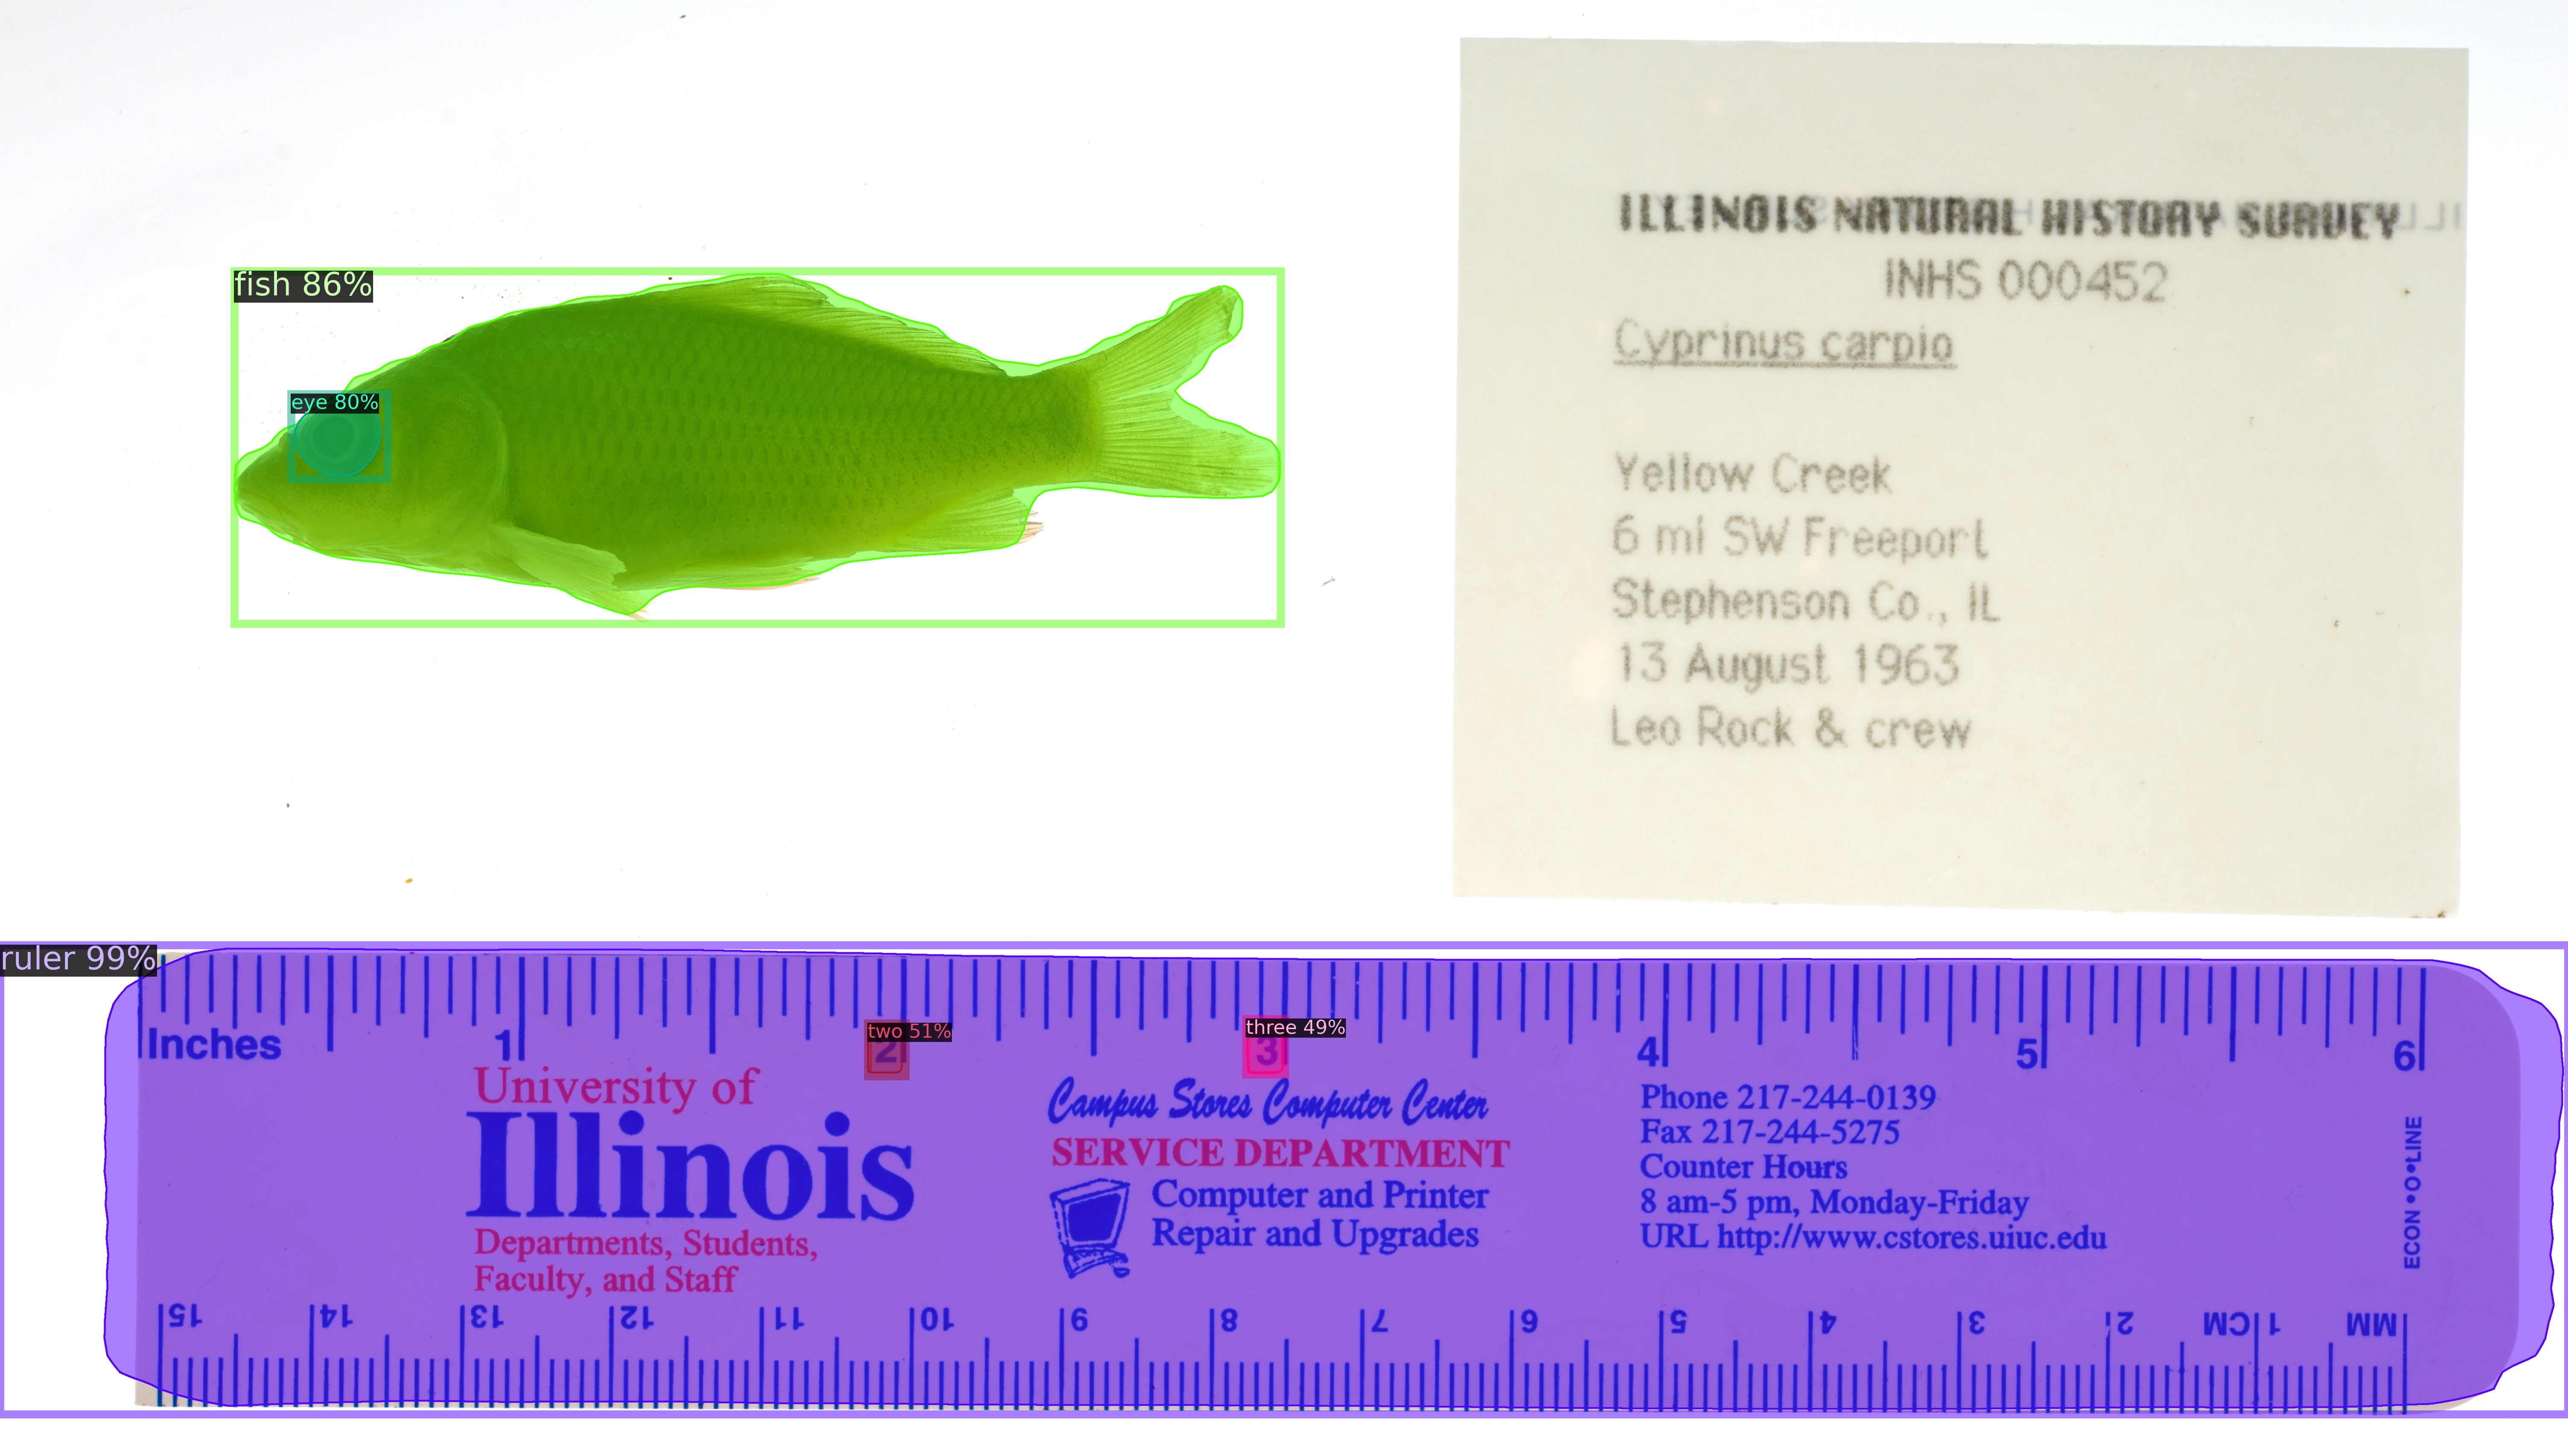
\includegraphics[width=.49\linewidth]{images/teaser1_crop}
  %\hspace{4mm}
  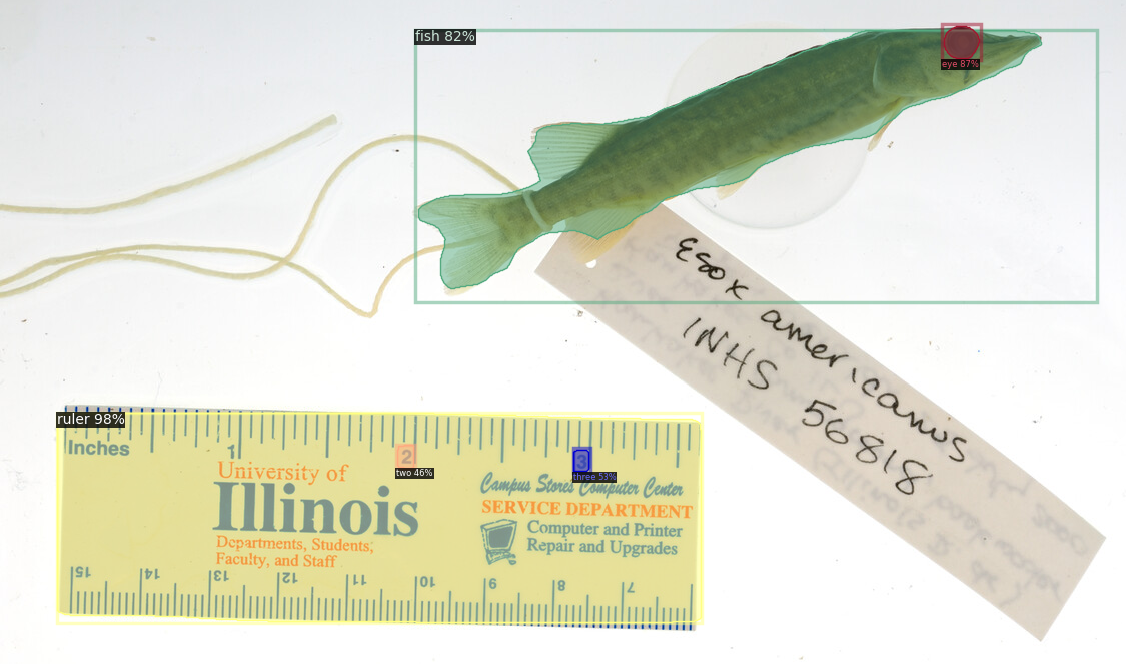
\includegraphics[width=.49\linewidth]{images/teaser2_crop}
  \caption{Initial object detection on specimen images using Detectron2~\cite{wu2019detectron2}}
  \label{fig:teaser}
\end{figure}
\subsection{Detectron}
A prerequisite task to performing any advanced metadata property generation
is finding the specimens (and other relevant objects) within the collection
images. Object detection has been a broadly active field of study in recent
years \cite{zou2019object}, and has resulted in a number of well-tested, purpose-built architectures. We elected to use Facebook AI Research's \verb|detectron| tool \cite{wu2019detectron2}, and specifically its implementation of the Mask R-CNN architecture \cite{he2018mask}, for object detection in our project.
\verb|detectron| is built on \verb|pytorch|~\cite{NEURIPS2019_9015} and provides a relatively straightforward method for training on COCO~\cite{DBLP:journals/corr/LinMBHPRDZ14} format datasets. It is able to handle an arbitrary number of object classes, and can classify an arbitrary number of object within a given image. For our project, we are currently using it to identify five object classes: fish, fish eyes, rulers, and the numbers 2 and 3 on rulers.

% Not sure wrapping this is really getting us much after the 2 column switch

%\begin{wraptable}{r}{5.5cm}
\begin{table}[H]
    \centering
      \caption{Training dataset}
    \label{tab:dataset}
    \begin{tabular}{cc}
        \toprule
        \textbf{Class} & \textbf{Number of Instances}\\
        \midrule
        Fish & 297\\
        Ruler & 1496\\
        Eye & 456\\
        Two & 100\\
        Three & 100\\
      \bottomrule
    \end{tabular}
\end{table}
%\end{wraptable}

Table \ref{tab:dataset} lists the number of instances for each class 
used in our training dataset.
All of the training data was labeled by hand using \verb|makesense.ai| \cite{make-sense}
% While the ultimate goal of the project is to generalize to images from a variety of specimen collections, we have thus far focused only
on images from the INHS\ Fish Collection \cite{INHS}.
Using \verb|detectron|'s default training scheme, the model was trained for \(100,000\) epochs. All instance types were included in a single object detection model. The total loss\todo{Find and specify which loss function was used} began at \(2.948\) and ended at \(0.158\) for the training data.

\begin{comment}
\begin{verbatim}
|  category  | #instances   |  category  | #instances   |  category  | #instances   |
|:----------:|:-------------|:----------:|:-------------|:----------:|:-------------|
|    fish    | 297          |   ruler    | 1496         |    eye     | 456          |
|    two     | 100          |   three    | 100          |            |              |
|   total    | 2449         |            |              |            |              |

Iterations: 100,000

Initial: {"data_time": 0.004866079999999329, "fast_rcnn/cls_accuracy": 0.115234375,
"fast_rcnn/false_negative": 0.1686291000841043,
"fast_rcnn/fg_cls_accuracy": 0.2782012195121951, "iteration": 5, "loss_box_reg": 0.40475407242774963,
"loss_cls": 1.8559419512748718, "loss_mask": 0.6982034742832184, "loss_rpn_cls": 0.05218731239438057,
"loss_rpn_loc": 0.007734265644103289, "lr": 0.00011990000000000001, "mask_rcnn/accuracy": 0.2920252418802887,
"mask_rcnn/false_negative": 0.9506743610216735, "mask_rcnn/false_positive": 0.2467277275646746,
"roi_head/num_bg_samples": 115.0, "roi_head/num_fg_samples": 13.0, "rpn/num_neg_anchors": 251.25,
"rpn/num_pos_anchors": 4.75, "time": 0.2812129614999961, "total_loss": 2.9480794025585055}

Final: {"data_time": 0.006645713496254757, "eta_seconds": 0.0, "fast_rcnn/cls_accuracy": 0.984375,
"fast_rcnn/false_negative": 0.0, "fast_rcnn/fg_cls_accuracy": 1.0, "iteration": 99999,
"loss_box_reg": 0.054501257836818695, "loss_cls": 0.03908616118133068, "loss_mask": 0.06379510834813118,
"loss_rpn_cls": 0.0010549294238444418, "loss_rpn_loc": 0.005114196799695492, "lr": 0.02,
"mask_rcnn/accuracy": 0.9722937165937804, "mask_rcnn/false_negative": 0.012800597698663846,
"mask_rcnn/false_positive": 0.05609636495338312, "roi_head/num_bg_samples": 115.75,
"roi_head/num_fg_samples": 12.25, "rpn/num_neg_anchors": 246.5, "rpn/num_pos_anchors": 9.5,
"time": 0.3563086399990425, "total_loss": 0.15775199318886735}
\end{verbatim}
\end{comment}
\subsection{Pixel Analysis}
The masks and bounding boxes produced by \verb|detectron| are generally quite good, although they almost never completely or tightly enclose the
detected objects.
This is problematic for the detected fish objects in our analyzed images,
where the most accurate segmentation is desired.
The mask may include additional background as part of the fish, or the
bounding box may clip away part(s) of the fish. To solve these
shortcomings, we utilize pixel analysis methods commonly found in image
informatics to produce more accurate objects masks and bounding boxes.

\subsubsection{Threshold Adjustment}
The first calculation in the pixel analysis process determines the cutoff intensity between what constitutes the foreground (i.e.~the fish) and background of the image.
Initially, the calculation is based on the bounding box and mask generated by
\verb|detectron|. Specimen images are read in as gray scale, and pixels in the image are treated as unsigned integers between 0 and 255.
Otsu thresholding, a technique that maximizes the variance between the 
foreground and background intensities, is used to compute an initial cutoff value between foreground and background. 
While the Otsu value occasionally generates an accurate mask as is, usually
the contrast between foreground and background is low and much of the lighter parts of the fish (such as its tail fin) are marked as background.

To overcome this under-segmentation, the threshold value should be
either adjusted up or down, depending on if the background is lighter or darker than the fish.
For our current dataset, the background is always lighter (i.e.~closer to 255), so the threshold value needs to be scaled up to include more of the
foreground image.
% Precisely how much to scale this value by is difficult to determine.
For optimal results the scaling should be dependent on the
contrast between the background and foreground,
which can be affected by
% both how washed out the image is and
the level of pigmentation of the fish.
% To take this into account, we compute the mean intensity of the foreground and background pixels, then use these intensity values and the difference between them to scale the threshold value.
% Even with these values in hand it is not entirely clear how to scale the threshold.
We found that an improved threshold value can be computed as the halfway
point between the Otsu threshold value and the
mean of the background intensities.
This adjusted threshold value
% by 50\% of the difference between the mean of the background and the original threshold value, which 
captures most of fish's fins in most cases, without also masking parts of the background.

\subsubsection{Consolidating the Foreground}
While thresholding has the potential to generate better masks than a neural network (when provided an initial approximate bounding box), it also introduces considerable noise. Single or small groups of errant pixels can be marked as foreground depending on the consistency of the background, and interior pixels of the fish (especially around the fins) can be marked as background. To be useful for generating an accurate bounding box and for subsequent computational analysis, the mask must consist of one single ``blob'' over the fish the contains no holes, and no other pixels disconnected from this blob can be marked as foreground.

To accomplish this, we apply an iterative process of flood filling from all the foreground pixels in the image until a blob is generated that is large enough to constitute the fish. This is another metaparameter, but greater than 10\% of the current bounding box has masked the specimen in all observed cases. Once the fish's blob is found, noise then needs removed. This is done by flood filling from each of the corner of the bounding box where the specimen is not present (all four corners in the overwhelming majority of cases), then taking the inverse of the result. The fish mask is excluded from these corner flood fills, so this process removes all noise from both the background and foreground of the image leaving only a close mask over the fish itself.

\subsubsection{Adjusting the Bounding Box}
With an accurate mask generated, it is then necessary to check whether the bounding box needs expanded or shrunk along any edges. Expansion is done first, buy checking whether any edge intersects with any of the foreground mask pixels. If one does, it is expanded out by 1 pixel. If any edges are expanded, the whole the process, masking and expansion process is repeated to account for any changes in average intensities. Once no edges contain foreground pixels, the mask is the shrunk. This process is more efficient as all that is required is to shrink each edge by one up until the point they contain one or more foreground pixels. Once the shrinkage step is accomplished, the final mask and bounding box have been generated.

\subsubsection{Fallback} The pixel analysis process occasionally fails. This can occur if certain flood fill operations behave unexpectedly, or if the image is too washed out or otherwise atypical for the thresholding process to work correctly. In the event this happens, the original mask and bounding box generated by \verb|detectron| is used for metadata generation.
\subsection{Metadata Generation}
Including what has already been discussed, the following metadata properties are being currently being generated:

\begin{table*}[t]
    \centering
    \caption{Metadata properties}
    \label{tab:properties}
    \begin{tabular}{cccp{0.5\linewidth}}
        \toprule
        \textbf{Property} & \textbf{Association} & \textbf{Type} & \textbf{Explanation}\\
        \midrule
        \verb|has_fish| & Overall Image & Boolean & Whether a fish was found in the image.\\
        \verb|fish_count| & Overall Image & Integer & The quantity of fish present.\\
        \verb|has_ruler| & Overall Image & Boolean & Whether a ruler was found in the image.\\
        \verb|ruler_bbox| & Overall Image & 4 Tuple & The bounding box of the ruler (if found).\\
        \verb|scale| & Overall Image & Float & The scale of the image in \(\frac{\mathrm{pixels}}{\mathrm{cm}}\).\\
        \verb|bbox| & Per Fish & 4 Tuple & The top left and bottom right coordinates of what define the bounding box for a fish.\\
        \verb|background.mean| & Per Fish & Float & The mean intensity of the background within a given fish's bounding box.\\
        \verb|background.std| & Per Fish & Float & The standard deviation of the background within a given fish's bounding box.\\
        \verb|foreground.mean| & Per Fish & Float & The mean intensity of the foreground within a given fish's bounding box.\\
        \verb|foreground.std| & Per Fish & Float & The standard deviation of the foreground within a given fish's bounding box.\\
        \verb|centroid| & Per Fish & 4 Tuple & The centroid of a given fish's bitmask.\\
        \verb|primary_axis| & Per Fish & 2D Vector & The unit length primary axis (eigenvector) for the bitmask of a given fish.\\
        \verb|clock_value| & Per Fish & Integer & A fish's primary axis converted into an integer ``clock value'' between 1 and 12.\\
        \verb|length| & Per Fish & Float & The length of a fish in \(\frac{\mathrm{pixels}}{\mathrm{cm}}\).\\
        \verb|mask| & Per Fish & 2D Matrix & The bitmask of a fish in 0's and 1's.\\
        \verb|pixel_analysis_failed| & Per Fish & Boolean & Whether the pixel analysis process failed for a given fish. If \verb|true|, \verb|detectron|'s mask and bounding box were used for metadata generation.\\
        \verb|score| & Per Fish & Float & The percent confidence score output by \verb|detectron| for a given fish.\\
        \verb|has_eye| & Per Fish & Boolean & Whether an eye was found for a given fish.\\
        \verb|eye_center| & Per Fish & 2 Tuple & The centroid of a fish's eye.\\
        \verb|side| & Per Fish & String & The side (i.e.\ \verb|'left'| or \verb|'right'|) of the fish that is facing the camera (dependent on finding its eye).\\
      \bottomrule
\end{tabular}
\end{table*}

\verb|has_fish|, \verb|fish_count|, \verb|has_ruler|, \verb|ruler_bbox|, \verb|background.*|, \verb|foreground.*|, \verb|bbox|, \verb|mask|, \verb|score|, and \verb|has_eye| have already been discussed. The remaining properties are determined as follows:
\subsubsection{centroid and eye\_center}
Centroids are provided for masks/bounding boxes generated by \verb|detectron|, and since we do not recalculate the mask of fish eyes we can use that value directly for \verb|eye_center|.

Since we recalculate the mask of the fish, we must recalculate its centroid as well. This can be done via
\begin{equation}
    (\bar{x}, \bar{y}) = (\mathrm{round}(\frac{M_{10}}{M_{00}}), \mathrm{round}(\frac{M_{01}}{M_{00}}))
\end{equation}
where \(M_{00}\) is the pixel area of the fish's blob, \(M_{10}\) is the sum of all the \(x\) values of blob pixels, and \(M_{01}\) is the sum of all the \(y\) values of blob pixels.
\subsubsection{side}
Determining which \verb|side| of the fish is visible is predicated on finding its eye. If an eye is found, the sign of the \(x\) component of the vector from the centroid of the fish to the centroid of the eye specifies which side is up: negative for left and positive for right. This assumes the fish was photographed vertically, which is essentially always the case for all image collections our group has worked on.
\subsubsection{primary\_axis and clock\_value}
The \verb|primary_axis| of a fish can be calculated by taking the covariance\todo{I could explain this in more detail if necessary} of its blob in \(x\) and \(y\), which yields its principle eigenvector. This can be directly assigned to the property. If an eye is present, we specify this axis in the direction of the eye in relation to the fish's centroid.

Our team encoded this information as a ``clock value'' between 1 and 12 when recording it by hand. To convert \verb|principal_axis| to \verb|clock_value|, the sign of \(x\) and \(y\) on the principal axis are used to determine which Cartesian quadrant the fish is angles into relative to its centroid. Depending on this quadrant, we then dot product the principal axis with either \([-1,0]\), \([0,-1]\), \([1,0]\) or \([0,1]\) which correspond to 9, 6, 3 and ``0'' o'clock respectively. The resulting radian value is then converted to a polar displacement in clock value space, and added to the comparative clock value used in the dot product. This then gives the fish's clock value from 0 to \(11.\overline{9}\). Before recording as \verb|clock_value| in the output, the value is rounded to the nearest integer, and in the event of a 0 final result it is replaced with 12.
\subsubsection{scale and length}
\(\frac{\mathrm{pixels}}{\mathrm{inch}}\) can be calculated by measuring the distance between the digits 2 and 3 found on the ruler by \verb|detectron|. Converting this to \(\frac{\mathrm{pixels}}{\mathrm{cm}}\) gives the \verb|scale| metadata property as reported in the output.

For the fish \verb|length| property, it is necessary to determine the furthest points from the centroid of the fish in each direction. Since fish are normally measured in a straight line from their snout down the middle of their trunk, we project every pixel onto the major axis of the fish (as a line through its centroid) before checking the distance. This projection is done by intersecting the line through the point along the tangent of the principal axis and the aforementioned centroid--principal axis line. After checking every pixel, measuring the distance between the two furthest projected points gives the length of the fish in pixels. Multiplying this by \verb|scale| gives the fish \verb|length| in centimeters.
\begin{comment}
\subsection{Consideration}
Just gonna throw some caveats in here, might be its own section might not
\begin{itemize}
    \item Program falls back to using detectron mask and bbox for metadata generation in the event the mask generation/pixel analysis fails. Failure is defined as never finding a cohesive flood filled mask that covers more than 10\% of the detectron bbox initially. Can provide a statistic on how often this occurs.
\end{itemize}
\end{comment}
\section{Results}
Technicians employed by our team have manually generated the 22 metadata properties deemed crucial to the overall BGNN project~\cite{Leipzig2021.01.28.428644} for a large number of INHS images. \(20,699\) total entries were created by 13 technicians that spanned \(8,398\) unique images. Of these \(8,398\) images, \(7,244\) were both not part of the \verb|detectron| training set and meet our current admissibility criteria for what \verb|detectron| and the pixel analysis process can reliably handle. We ran the metadata extraction program on these \(7,244\) images. These properties did not include information on image scale, fish length, or fish bounding boxes. For these properties, a random sample of 50 specimens from the set of \(7,244\) were analyzed by hand for comparison.

Our automated process currently generates 7 of the 22 core metadata properties: \verb|if_fish| (\verb|has_fish|), \verb|fish_number| (\verb|fish_count|), \verb|if_ruler| (\verb|has_ruler|), \verb|specimen_angled| (\verb|clock_value|), \verb|specimen_view| (\verb|side|), \verb|brightness| (derived from \verb|background.mean| and \verb|foreground.mean|), and \verb|if_background_uniform| (\verb|background.std|). In addition, our process also calculates bounding boxes and fish lengths in centimeters.\todo{Talk more about what we can and can't verify and how.}

\subsection{Fish Detection}
All images in the INHS dataset contain exactly one fish. For \(7,209\) of the specimen images, one fish was detected. For 25 of the images, 2 fish were detected, 3 fish were detected for 3 images, and for 7 images no fish were found. In the case of greater than 1 fish, 9 of the 28 contained tags which overlapped the fish and were themselves labeled as a second fish. Of the remaining 17, \verb|detectron| erroneously labeled the fish as two separate fish objects, or labeled a subsection of the fish a second time.

\subsection{Ruler Detection}
For all but 2 of the \(7,244\) images \verb|detectron| was able to find the ruler.\todo{Not sure if I can phrase it that way or not since I haven't looked at all the images to see if the ruler itself was found or something else was labeled a ruler} For an additional 56 images, the ruler itself was found but the ``2'' and/or the ``3'' on it was not, so a scale calculation could not be performed.

\subsection{Side Detection}
For 246 of the images \verb|detectron| was unable to find a fish eye. Of the remaining \(6,998\) images where it did, the correct side (\verb|left| or \verb|right|) was detected in all but 6 cases.

\subsection{Clock Value}
Clock position values were successfully generated for \(6,991\) of the images. Of those, all but 8 were within \(\pm{}1\) of the correct result.

\subsection{Brightness/Uniformity Results?}
\begin{verbatim}
Mean intensity in bounding box | Count

dark: 153.94935240158551 | 1800
normal: 168.2924981358199 | 5186
bright: 177.68854540643943 | 242
\end{verbatim}
\begin{verbatim}
Standard Deviations for:
    Uniform: 12.554834863869324
    Not Uniform: 11.312181711328828
\end{verbatim}

\subsection{Mask and Bounding Box}
\begin{figure}[H]
  \centering
  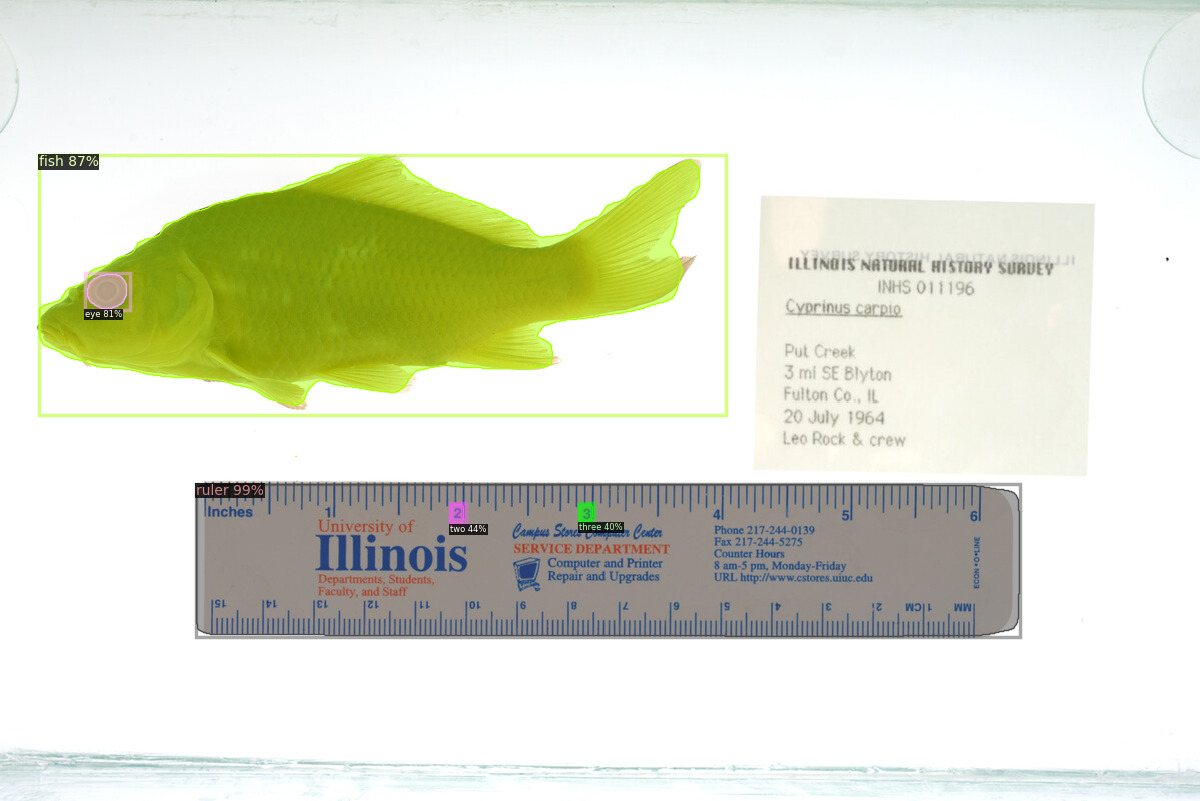
\includegraphics[width=0.49\linewidth]{images/011196_pred}
  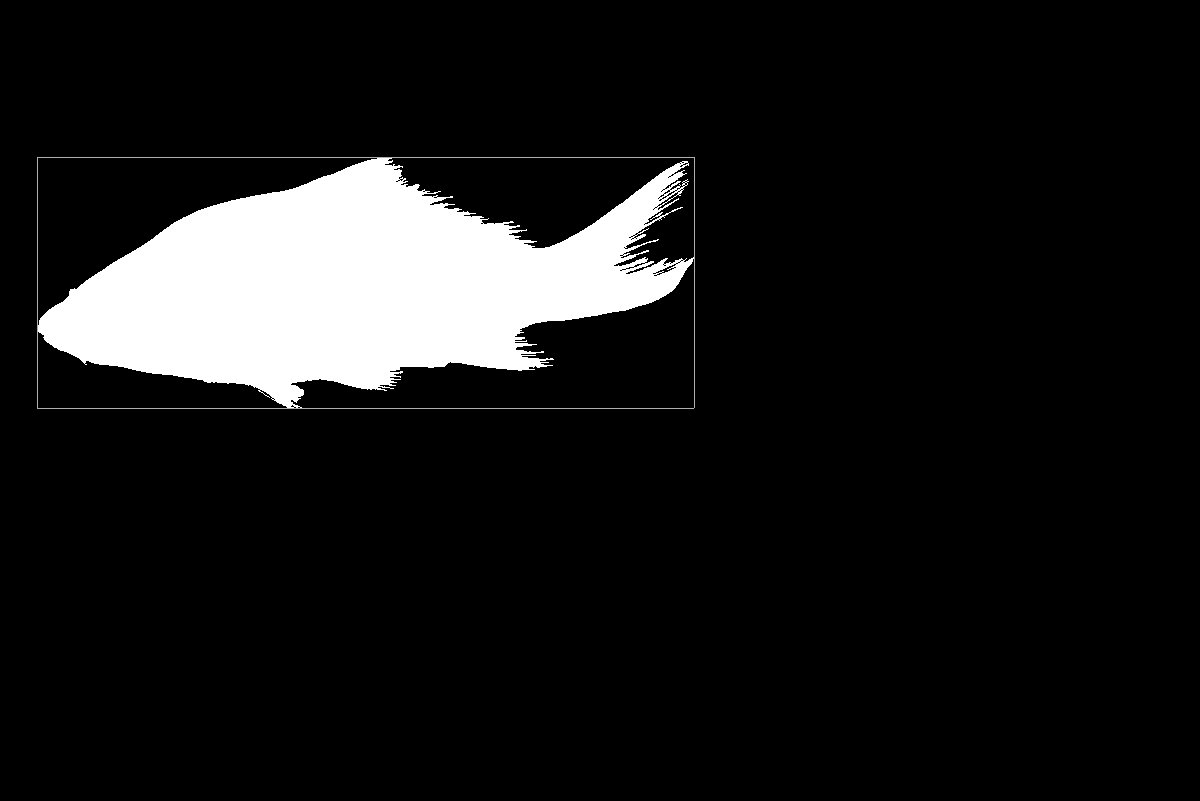
\includegraphics[width=0.49\linewidth]{images/011196_mask}
  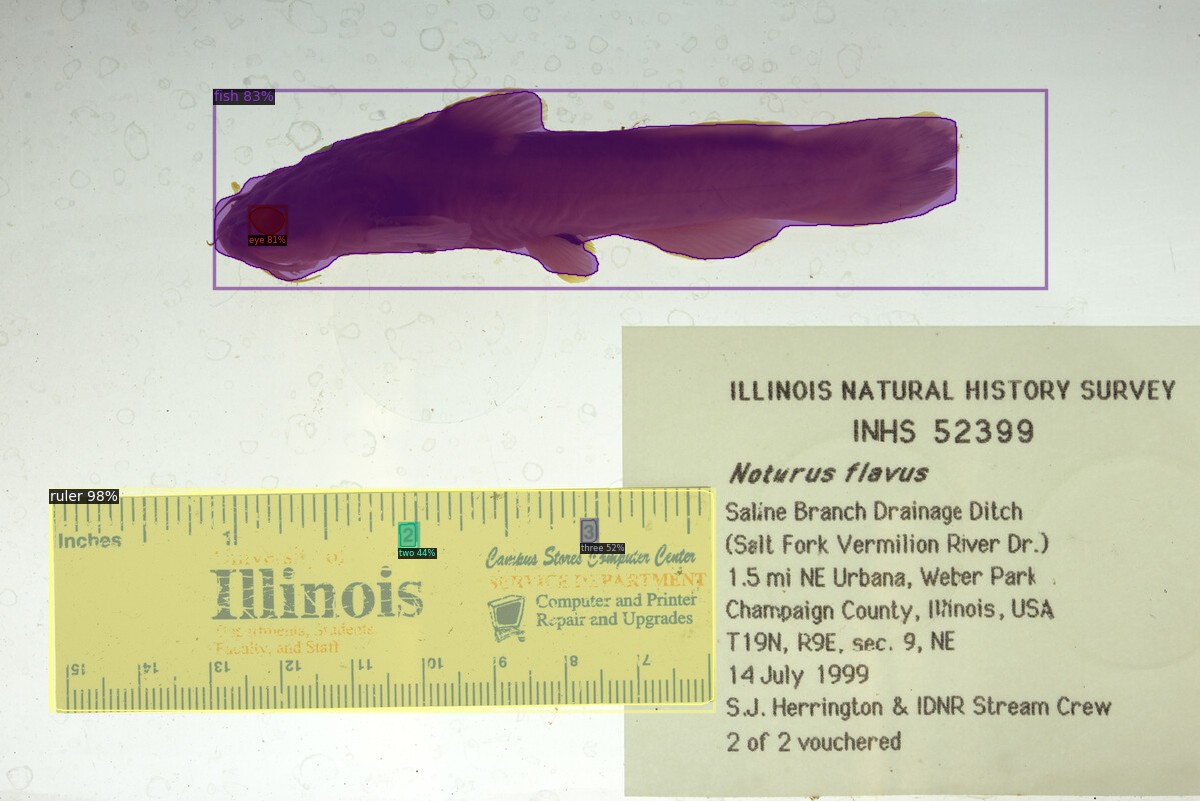
\includegraphics[width=0.49\linewidth]{images/52399_pred}
  
\includegraphics[width=0.49\linewidth]{images/52399_mask}
  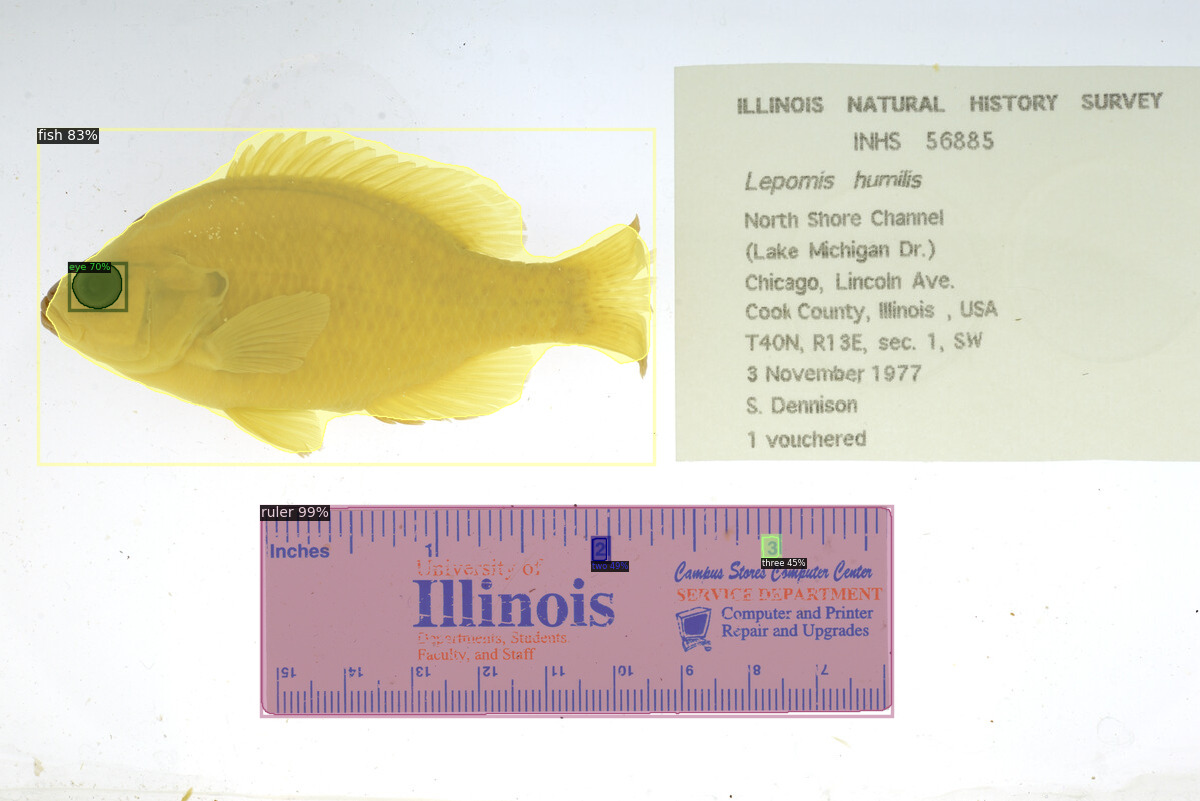
\includegraphics[width=0.49\linewidth]{images/56885_pred}
  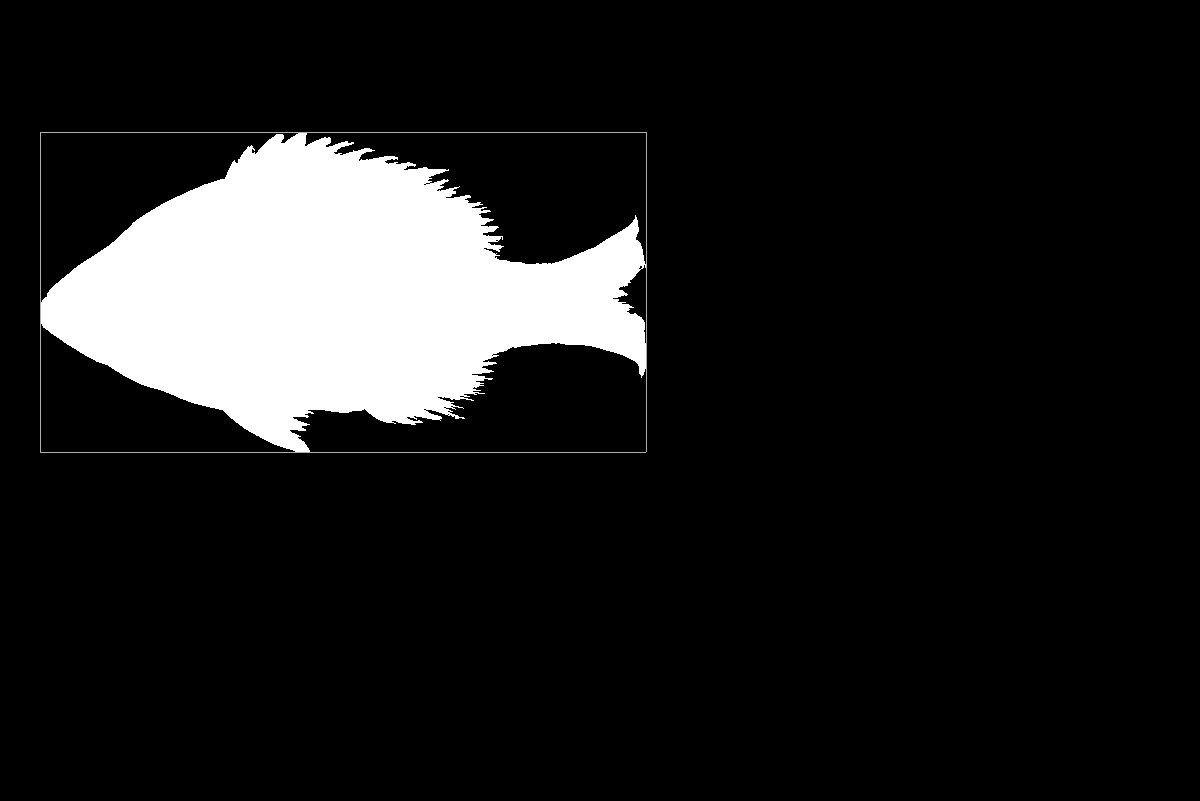
\includegraphics[width=0.49\linewidth]{images/56885_mask}
  \caption{Examples of masks and bounding boxes from detectron (left) and pixel analysis (right).}
\end{figure}
Fish bounding boxes were calculated for all \(7,237\) images in which a fish was found. All but 263 of these were generated via pixel analysis, with those 263 falling back to the original \verb|detectron| bounding box. Of the 50 images reviewed manually for these properties, all mask and bounding boxes were correctly placed on/around the location of the fish. However, a number of them lacked portions of lightly colored tails and/or fins. Specifically, 22 mask and bounding boxes covered the entire fish, 16 missed some of the tail, and 12 missed most or all of the tail.

\subsection{Scale and Length}
Image scale and fish lengths were calculated for \(7,179\) of the images. 50 of these images were measured by hand to get \(\frac{\mathrm{pixels}}{\mathrm{cm}}\) and fish length in centimeters with ImageJ.~\cite{imagejCite} The average error for the scale calculation was \(0.911\%\), and the average error for the fish length calculation was \(5.87\%\).

\section{Discussion}
\textbf{Todo}: Will need some sort of intro/framing paragraph
\subsection{Results}\todo{Just going to put the results discussion in small sections and we can change it later if that doesn't make sense}
\subsubsection{Object Detection}
\begin{figure}[H]
  \centering
  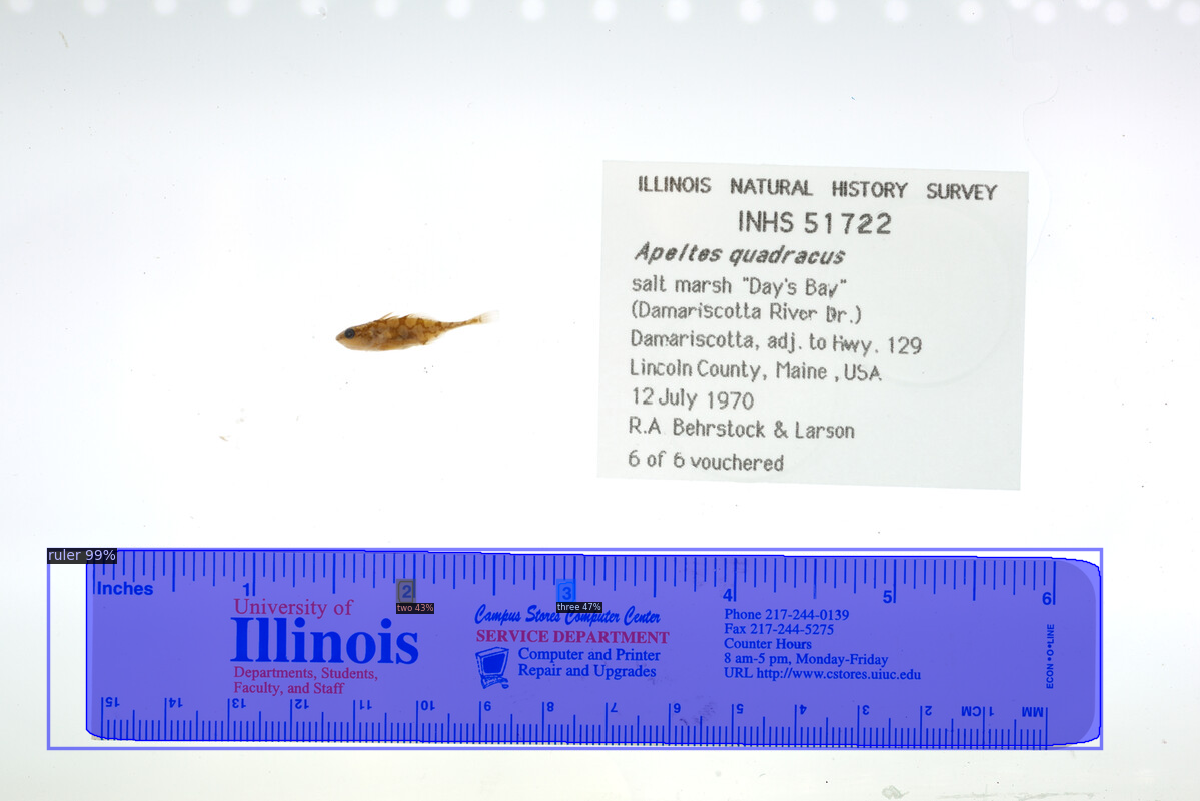
\includegraphics[width=0.49\linewidth]{images/none1}
  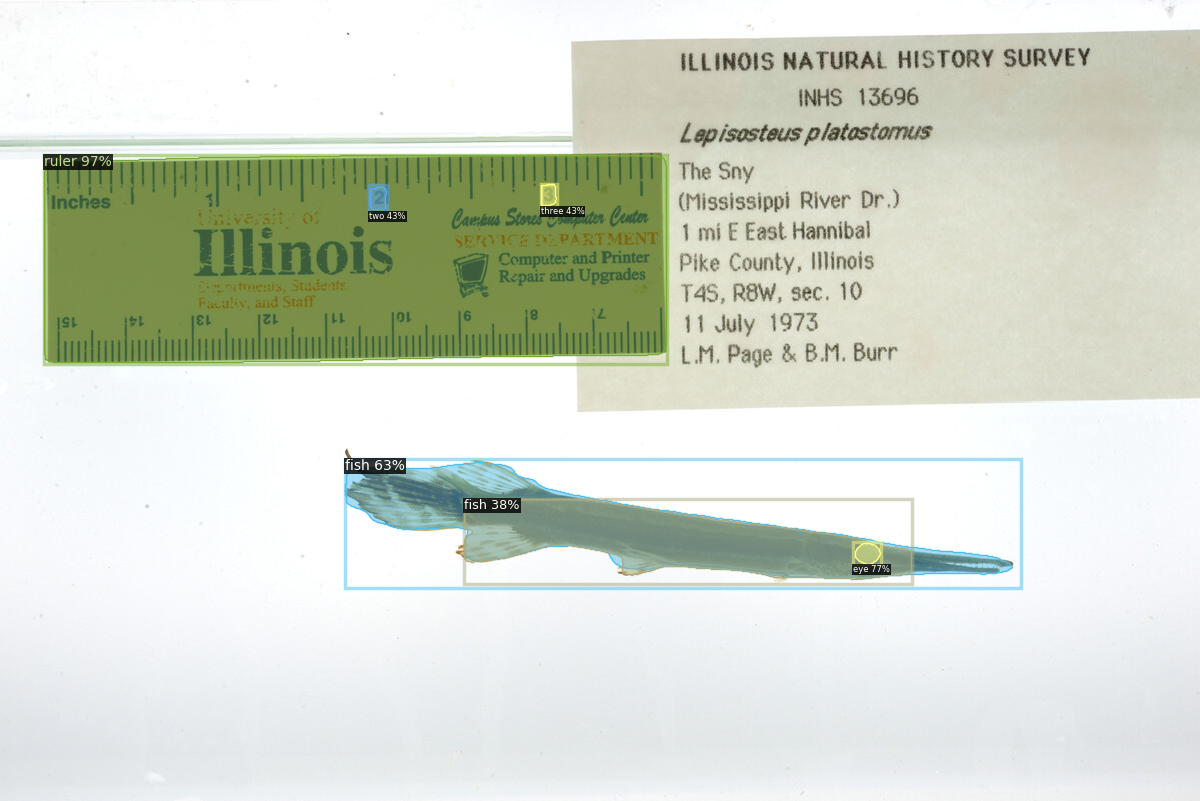
\includegraphics[width=0.49\linewidth]{images/double1}
  \caption{An example of a fish that was not detected (left) and a fish that was detected twice (right).}
\end{figure}

\begin{itemize}
    \item Worked fairly well all things considered
    \item Talk about which fish failed
    \item Talk about which rulers failed
\end{itemize}
\subsubsection{Side Detection}
\begin{figure}[H]
  \centering
  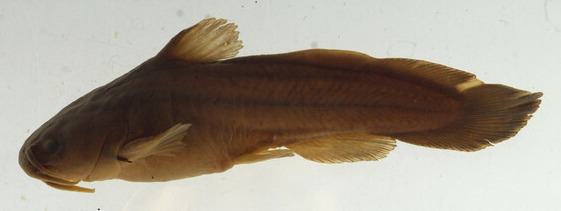
\includegraphics[width=0.49\linewidth]{images/wrong_side_orig}
  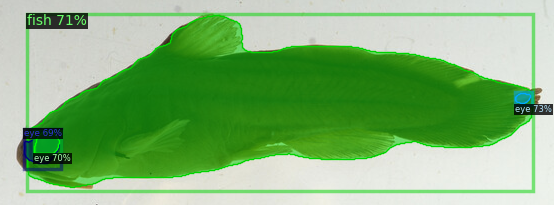
\includegraphics[width=0.49\linewidth]{images/wrong_side1}
  \caption{A fish for which a splotch on its tail fin was labeled the most likely eye.}
\end{figure}
For all 6 of the cases where an eye was detected but the \verb|side| value was wrong, a spot on the wrong side of the fish was labeled as the most likely eye within the bounding box of the fish. There were an additional 17 images for which the automated process generated a result that did not match the manually created data. For these remaining cases the manual data was incorrect, giving the automated system an error rate \(2.8\) times lower than than the human error rate.

\subsubsection{Clock Value}
\begin{figure}[H]
  \centering
  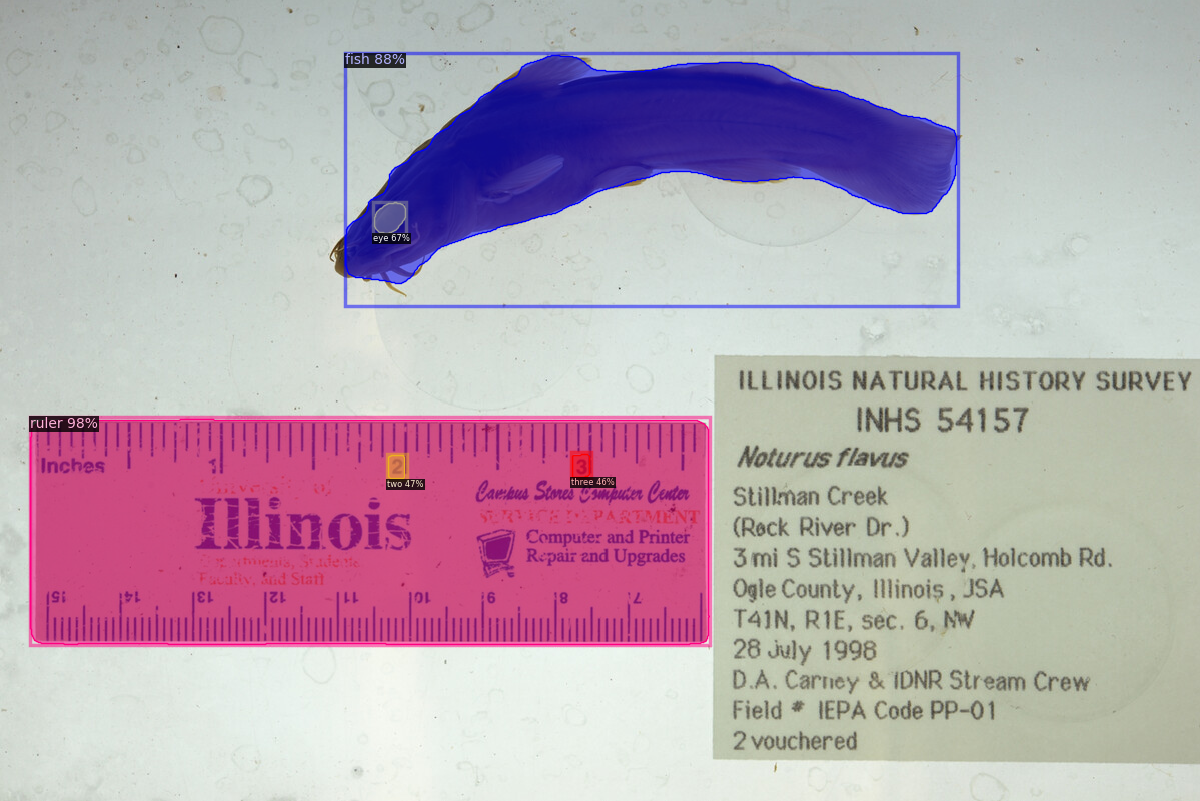
\includegraphics[width=0.49\linewidth]{images/curved1}
  \caption{An example of a heavily curved specimen.}
\end{figure}
Of the specimens for which clock values were generated, 33 did not match the manually created data (within a tolerance of \(\pm{}1\)).For 25 of those the human generated data was incorrect, giving the automated process a \(3.1\) times lower error rate. Of the remaining 8, 2 specimens were quite curved making it difficult to assign a clear angle value. The other 6 were values of 3 instead of 9 or vice versa that resulted from a mislabeled eye as discussed in the previous section. A small number of images (such as on the right in Figure~\ref{fig:teaser}) have tags that overlap with the fish. These tags were light enough that they were correctly labeled as background by the pixel analysis.

\subsubsection{Mask and Bounding Box}
\begin{figure}[H]
  \centering
  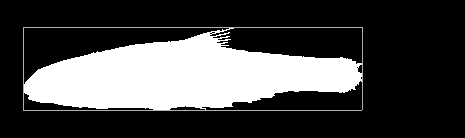
\includegraphics[width=0.49\linewidth]{images/61631}
  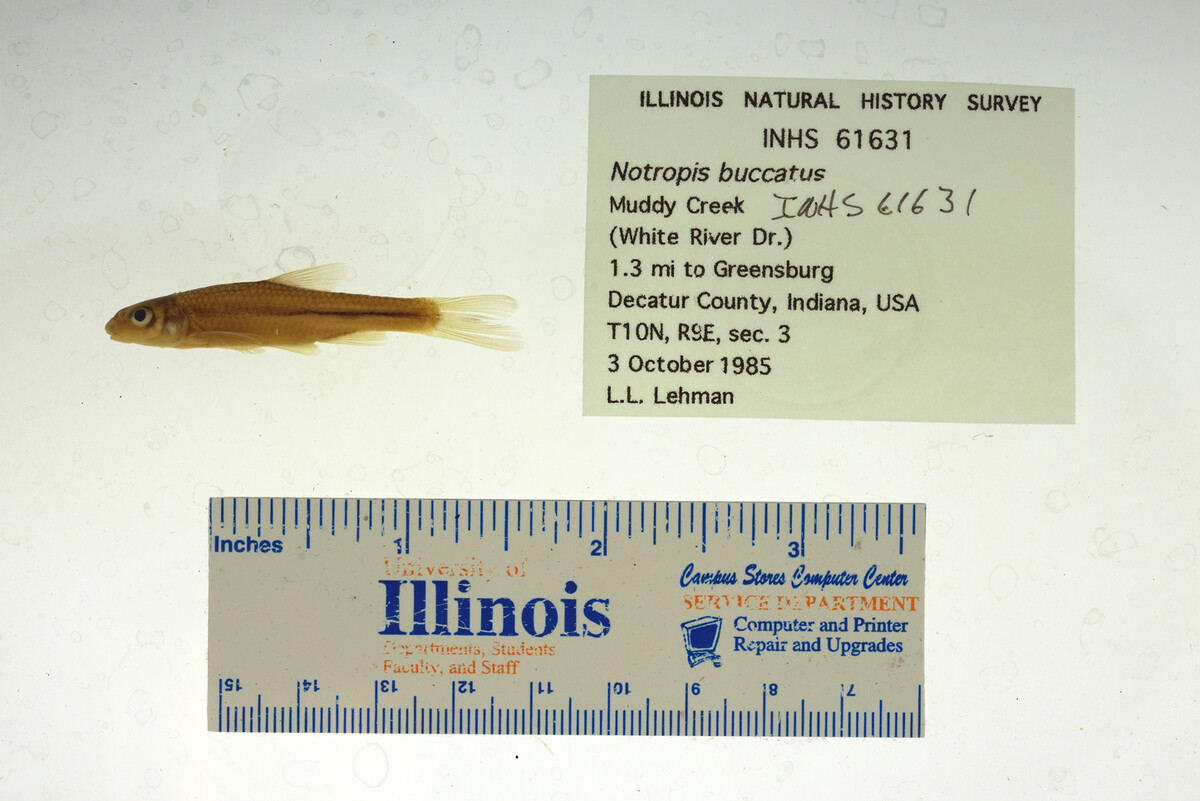
\includegraphics[width=0.49\linewidth]{images/61631_mask}
  \caption{An example of a light colored tail being missed during the pixel analysis process.}
\end{figure}
Masks and bounding boxes contain the head and trunk of the fish in nearly all cases, but there is still more fine tuning to be done to ensure that light fins and tails are masked consistently and accurately.\todo{Talk about ideas for fixing here, or in future work? Or both?}

\subsubsection{Brightness?}
\textit{Like I said in slack, the standard deviation of background does not currently correlate with the is\_background\_uniform property. Brightness results are are in previous section. Need to think about what is worth noting since it's a fairly trivial result.}

\subsubsection{Scale and Length}
\begin{figure}[H]
  \centering
  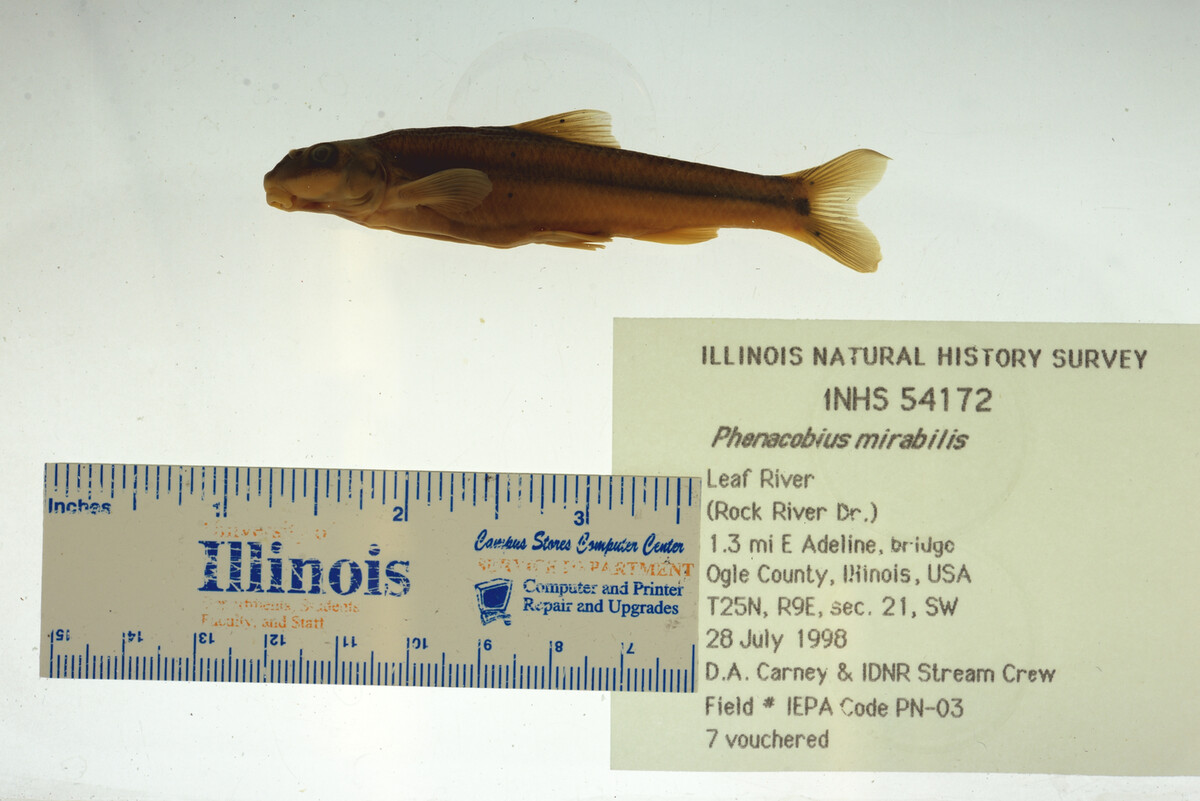
\includegraphics[width=0.49\linewidth]{images/54172}
  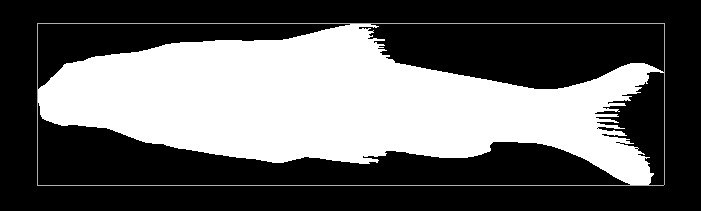
\includegraphics[width=0.49\linewidth]{images/54172_mask}
  \caption{An example of a light colored tail being missed during the pixel analysis process.}
  \label{fig:scale_len}
\end{figure}
Scale calculations using the ``2'' and ``3'' method are nearly identical to those calculated by hand between the tick marks on the ruler. When the tail of the fish is accurately masked and the specimen is fairly straight, the length calculation is highly accurate as well. An example of such a result can be seen in Figure~\ref{fig:scale_len}, for which the difference between the hand measured length and the automatically calculated length was only \(0.6\%\) (\(8.88\) cm vs \(8.82\) cm). Thus, the primary means of lowering the error of the length calculation is to improve tail masking accuracy.

\subsection{Future Work}
The most pressing next step is to refine the pixel analysis thresholding process so that the entirety of even light colored fish are marked as foreground in the mask. A deficiency of the current process is that it only operates on single channel intensity. Some of the lightest tails appear yellow in hue to the human eye and easily distinguishable, but when compressed to a single intensity value they are almost identical in value to the white background. Considering when the RGB channels of a pixel are not equal in value may be able to improve masking of such features. Another possible approach to solving this is to threshold an mask on subsets of the bounding box, as to ensure that very dark trunk pixels do not affect the thresholding of lighter regions.

Our ultimate goal is to create a generalized process to work on classes of specimen images (specifically all fish images for BGNN), not only the INHS collection. To accomplish this, a much larger training dataset full of more diverse images will be required. Another requirement will be to generalize the ruler reading process beyond the INHS specific reading of digits on the ruler.\todo{Suggest way(s) to do this?}
% Todo: Are these worth mentioning?
%Adding things like seahorses and eels.
%Fitting a ``spine'' to specimen.
\section{Conclusion}
\textbf{Todo}

\section*{Acknowledgment}

Vishal? Hank's undergrads? Other team members?

\bibliographystyle{IEEEtran}
\bibliography{paper}

\end{document}

%\begin{table}[htbp]
%\caption{Table Type Styles}
%\begin{center}
%\begin{tabular}{|c|c|c|c|}
%\hline
%\textbf{Table}&\multicolumn{3}{|c|}{\textbf{Table Column Head}} \\
%\cline{2-4} 
%\textbf{Head} & \textbf{\textit{Table column subhead}}& \textbf{\textit{Subhead}}& \textbf{\textit{Subhead}} \\
%\hline
%copy& More table copy$^{\mathrm{a}}$& &  \\
%\hline
%\multicolumn{4}{l}{$^{\mathrm{a}}$Sample of a Table footnote.}
%\end{tabular}
%\label{tab1}
%\end{center}
%\end{table}

%\begin{figure}[htbp]
%\centerline{\includegraphics{fig1.png}}
%\caption{Example of a figure caption.}
%\label{fig}
%\end{figure}
